\newpage
\section{It Takes All Kinds\dots}\label{A:otherCurves}
\fixnote{Maybe move these to problems.  Replace with linear, quadratic, exponential sheet.}

Data can come in all shapes and sizes. While a line is the simplest
approximation, it might not be the best.

\begin{prob}
Consider the data below:
\[
\begin{array}{|c|c|c|c|c|}\hline
x & 0 & 1 & 2 & 3 \\ \hline
y & 8.1 & 22.1 & 60.1 & 165 \\ \hline
\end{array}
\]
What type of data is this? To get the ``brain
juices'' flowing here are some choices. It could be:
\begin{enumerate}
\item A parabola.
\item An exponential.
\item A quartic.
\item Something else.
\end{enumerate}
Hint: Think about the most famous graph of all, the one you know most
about.  And see if you can somehow convert the above data to get that
type of graph. You will probably need to make some plots. 
\end{prob}


\begin{prob}
Now do the same with this data:
\[
\begin{array}{|c|c|c|c|c|}\hline
x & 1 & 2 & 3 & 4 \\ \hline
y & 8.3 & 443.6 & 24420.8 & 1364278.6 \\ \hline
\end{array}
\]
\end{prob}


\begin{prob}
Now do the same with this data:
\[
\begin{array}{|c|c|c|c|c|c|}\hline
x & 1 & 2 & 3 & 4 & 5 \\ \hline
y & 7 & 62 & 220 & 506 & 1012 \\ \hline 
\end{array}
\]
\end{prob}

\begin{prob}
Here is a sample of semi-log paper. What's going on here?
\[
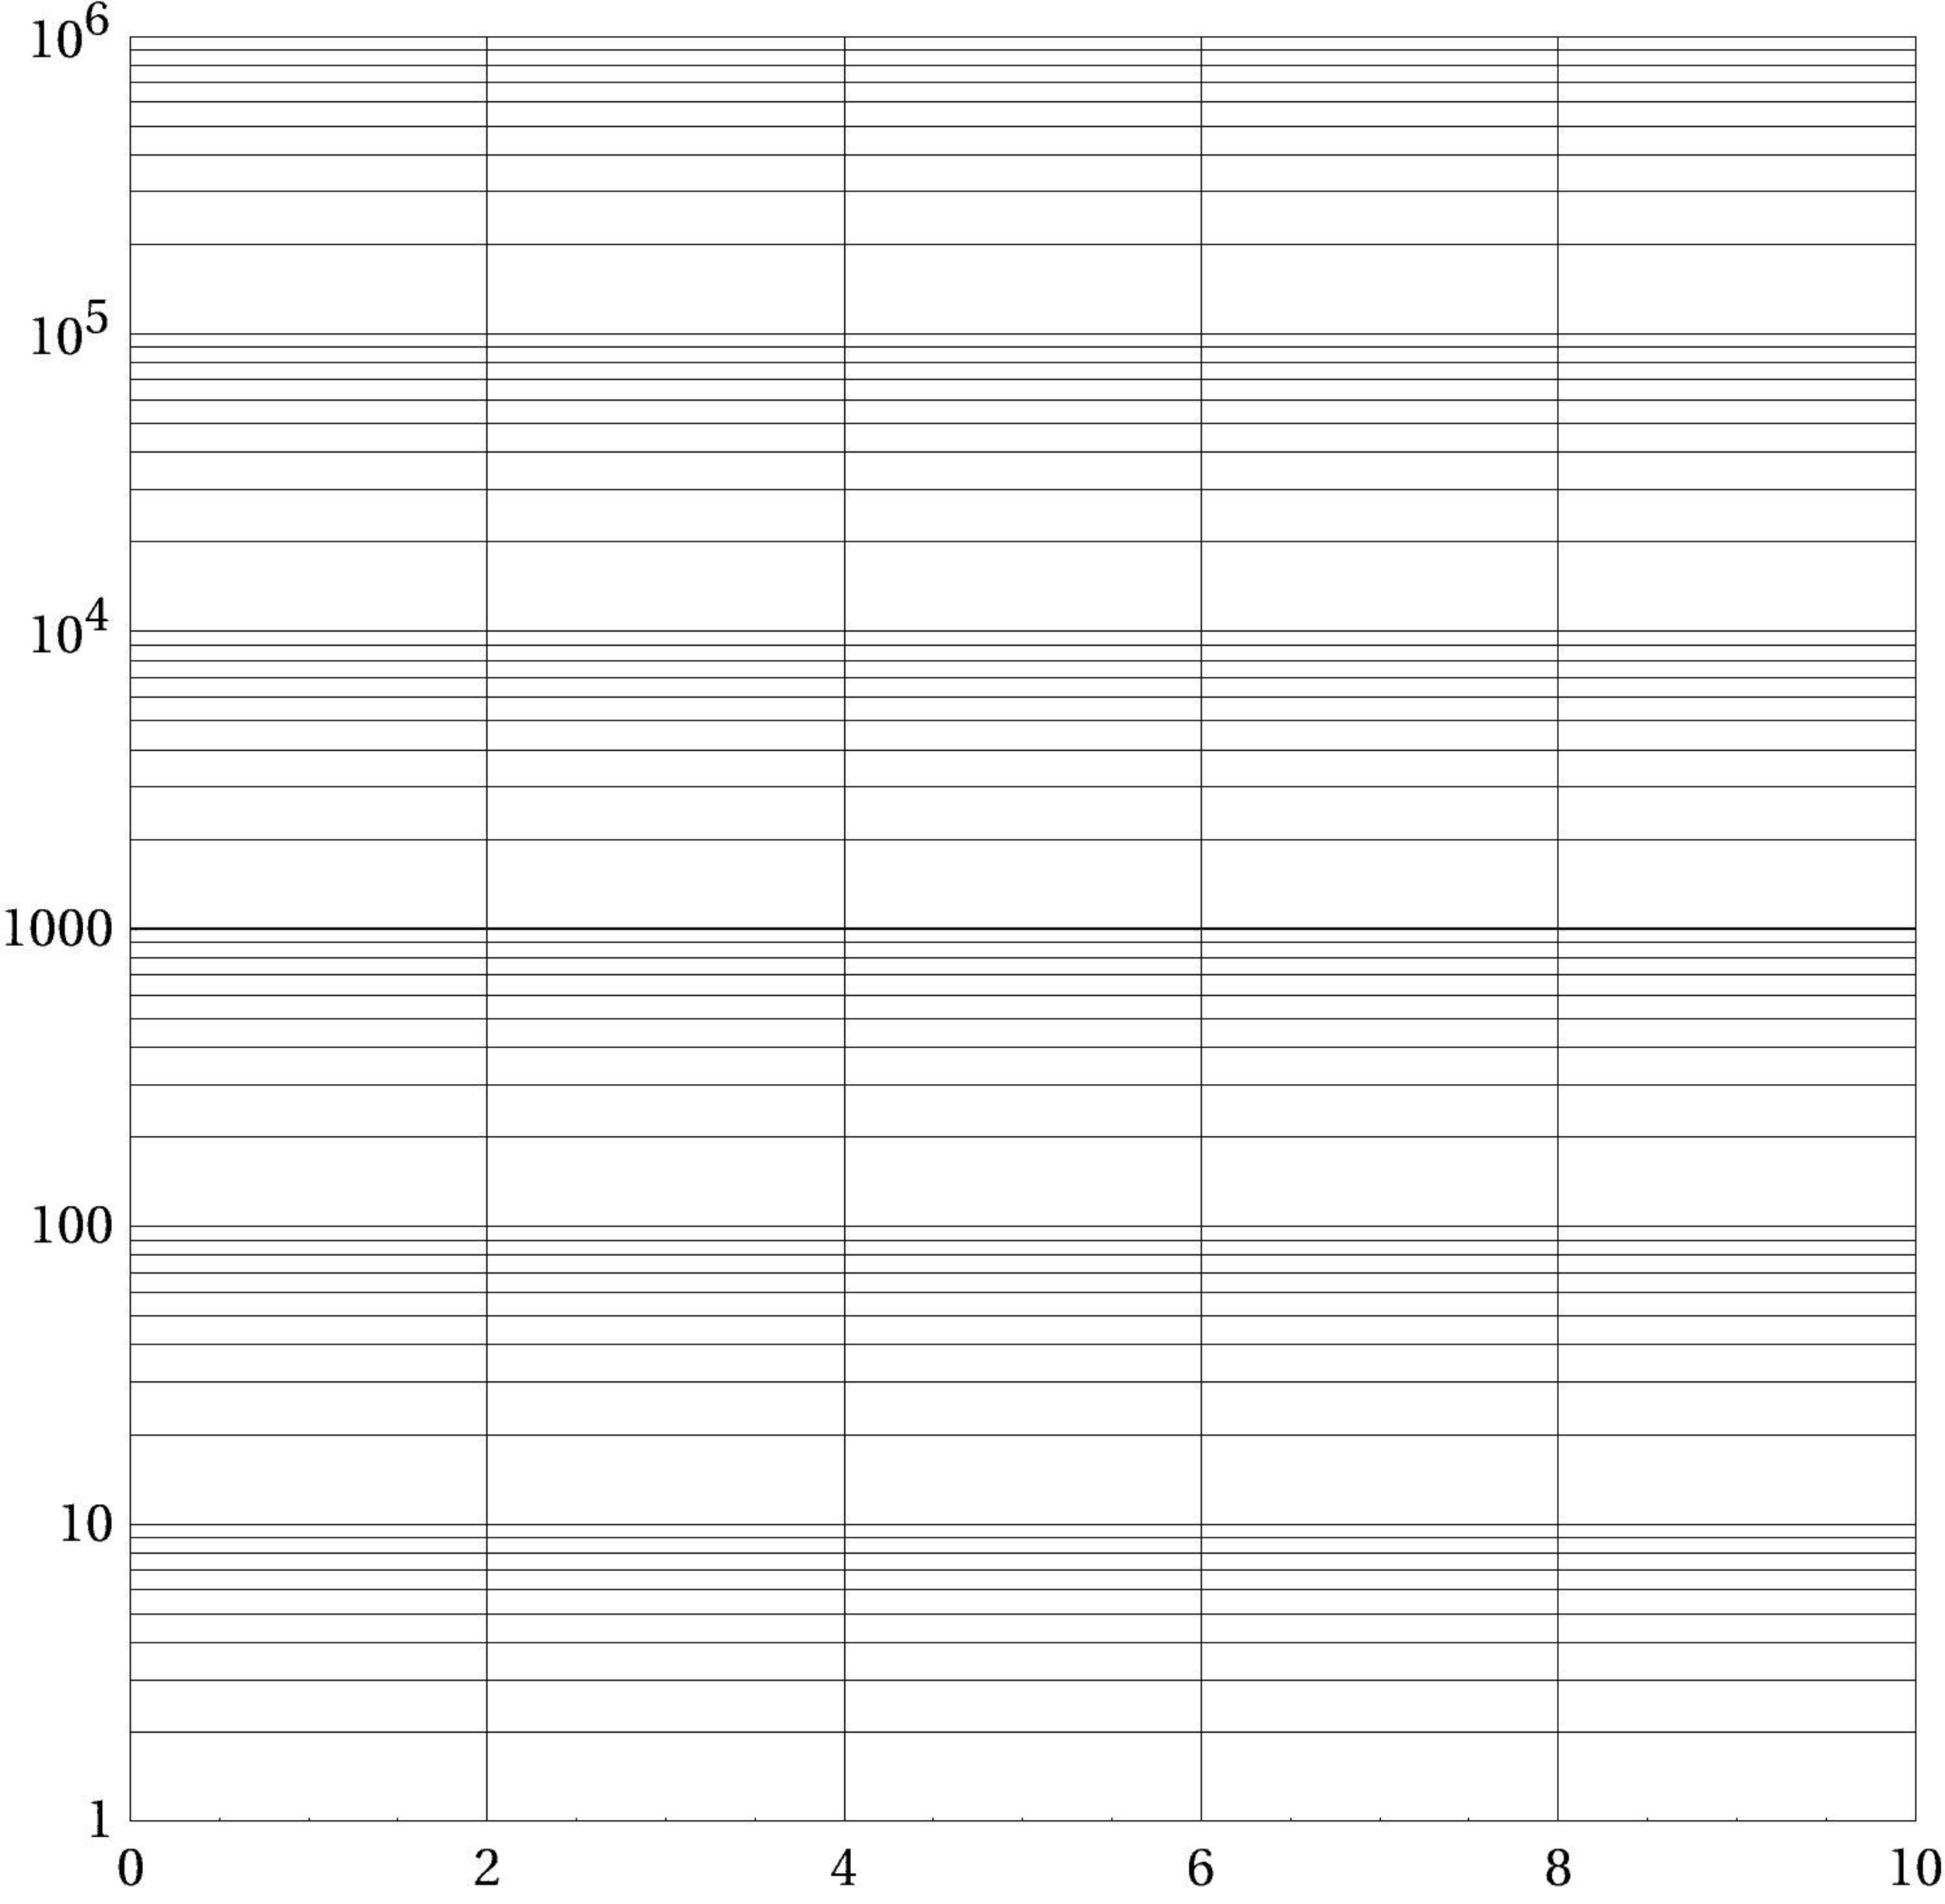
\includegraphics[width=4in]{../graphics/semiLog.pdf}
\]
\end{prob}
